\chapter{الدم والجملة الدورانية}\label{ch:b2:blood-circulation}

سنة 1628 أجرى وليام هارفي حسابًا. فالقلب، كما قدّر، يسع
نحو أوقيتين من \omterm{def:b2:blood-circulation:blood}{الدم} وينبض سبعين مرة في الدقيقة؛ وحتى لو
لم يُقذف من ذلك إلا كسر في كل نبضة، لضخّ القلب
في ساعة أضعاف وزن الجسم كله. ولا يمكن أن
يُصنع \omterm{def:b2:blood-circulation:blood}{الدم} ويُستهلك بذلك المعدل، كما علّم جالينوس
أربعة عشر قرنًا؛ فلا بد أن يدور ويدور. ثم
بيّن ذلك: اربط خيطًا حول الذراع فتنتفخ الأوردة أسفل
الخيط لا أعلاه؛ وادفع \omterm{def:b2:blood-circulation:blood}{الدم} في \omterm{def:b2:blood-circulation:vessels}{وريد} نحو اليد، عابرًا
دسامًا، فلن يمضي. \omterm{def:b2:blood-circulation:blood}{فالدم} يُضخ خارجًا عبر
الشرايين، ويعود عبر الأوردة، وتمر اللترات الخمس كلها
عبر القلب كل دقيقة. وهذا الفصل عن تلك الجملة المغلقة
--- ما \omterm{def:b2:blood-circulation:blood}{الدم}، وكيف يُوجَّه، وفيزياء جريانه
في الأوعية من الأبهر إلى \omterm{def:b2:blood-circulation:vessels}{شعيرة}، و
التبادل، في الشعيرات، الذي هو الغاية من ذلك كله.

\section{الدم}

\begin{definition}[تركيب الدم]\label{def:b2:blood-circulation:blood}
\index{دم}\index{بلازما}\index{هيماتوكريت}\index{كرية حمراء}\index{صفيحة دموية}
الدم نسيج في معلق: نحو \qty{5}{L} عند البالغ، أي
\qty{7}{\%} من كتلة الجسم. وبالطرد المركزي ينفصل إلى
\emph{بلازما} (\qty{55}{\%}: ماء، و\qty{70}{g/L} من البروتينات ---
الألبومين، والغلوبيولينات، والفيبرينوجين --- والأملاح والسكريات والشحوم
والغازات والهرمونات التي تحملها) وخلايا (\qty{45}{\%}، وهي
\emph{الهيماتوكريت}): \emph{كريات حمر} ($5\times 10^{12}$ في اللتر،
وهي أقراص مقعرة الوجهين بقطر \qty{7}{\micro m} بلا نواة، محشوة كل منها
بعدد \num{280} مليون جزيء هيموغلوبين، تعيش 120 يومًا و
تُصنع في النقي بمليونين في الثانية)، و\emph{كريات بيض}
($7\times 10^{9}$ في اللتر: عدلات، ولمفاويات، ووحيدات،
وحمضات، وأسسات، وهي الذراع المتحركة للمناعة)، و
\emph{صفيحات} ($3\times 10^{11}$ في اللتر، وهي شظايا من خلايا
النقي تسد الجروح وتبدأ التخثر). والكريات الحمر تحمل
الأكسجين --- \qty{200}{mL} في لتر الدم عند الإشباع التام،
أي سبعين ضعف ما يذيبه الماء --- وتحمل البلازما
كل ما سواه، بما فيه \qty{20}{\%} من $\mathrm{CO_2}$ التي
ليست في الخلايا، وحرارة العضلات إلى الجلد، و
هرمونات \cref{ch:b2:cell-signalling} إلى أهدافها. والدم
كذلك محلول تحت \emph{\omterm{thm:b2:blood-circulation:oncotic}{ضغط غرواني}}: فبروتيناته،
التي لا تستطيع مغادرة الشعيرات، تمسك نحو \qty{25}{mmHg} من
الجذب التناضحي، وذلك الجذب هو الذي يبقي البلازما في
الأوعية.
\end{definition}

\begin{omfigure}
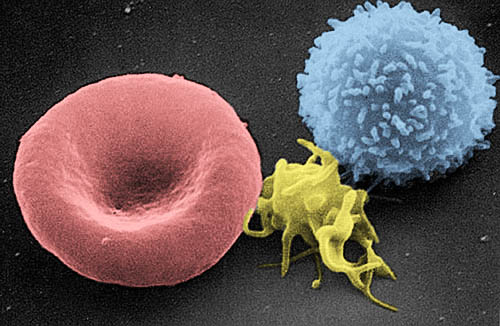
\includegraphics[width=0.5\linewidth]{images/book3/red-cells-nci.jpg}

{\small \omterm{def:b2:blood-circulation:blood}{كرية حمراء} وصفيحة وكرية بيضاء (لمفاوية)
تحت المجهر الإلكتروني الماسح: مكونات \omterm{def:b2:blood-circulation:blood}{الدم} الخلوية
الثلاثة، مرسومة بالمقياس نفسه.}
\end{omfigure}

\begin{proposition}[الإرقاء]\label{prop:b2:blood-circulation:clotting}
\index{إرقاء}\index{شلال التخثر}\index{فيبرين}
يُسد الوعاء المقطوع بثلاث خطوات في دقائق. فينقبض الوعاء؛
وتلتصق الصفيحات بالكولاجين المكشوف، وتطلق
إشارات تجنّد صفيحات أخرى وتنشّطها، فتكوّن سدادة؛
و\emph{شلال} من بروتيازات \omterm{def:b2:blood-circulation:blood}{البلازما}، ينشّط كل منها التالي
(اثنا عشر عامل تخثر، معظمها مصنوع في الكبد، وعدة منها يحتاج إلى
فيتامين K)، يحوّل الفيبرينوجين إلى \emph{فيبرين} غير منحل، تشبك
خيوطه السدادة خثرةً. والشلال يضخّم: فأثر من
المنبه (عامل نسيجي من الجدار المتضرر) ينتهي إلى غرامات من
الفيبرين. ولا بد أيضًا من احتوائه: فمضادات التخثر في \omterm{def:b2:blood-circulation:blood}{البلازما}
(مضاد الثرومبين، والبروتين C) وعلى البطانة السليمة تحصر
الخثرة في الجرح، وتحلها جملة ثانية، هي حل الفيبرين،
مع التئام الوعاء. والناعور فقد عامل واحد؛ و
الخثار خثرة حيث لا تُراد، والسبب الأول
للوفاة في البلدان الغنية خثرة في \omterm{def:b2:blood-circulation:vessels}{شريان} إكليلي أو دماغي.
\end{proposition}

\section{الدارات}

\begin{definition}[مفتوحة ومغلقة، مفردة ومضاعفة]\label{def:b2:blood-circulation:circuits}
\index{دوران مفتوح}\index{دوران مغلق}\index{دوران مضاعف}\index{دوران رئوي}\index{دوران جهازي}
في الدوران \emph{المفتوح} (الحشرات، ومعظم الرخويات) يضخ قلب
\omterm{def:b2:blood-circulation:blood}{الدم} إلى جوف الجسم حيث يغمر الأعضاء مباشرة و
يعود بضغط منخفض؛ والجريان بطيء رديء التوجيه، وقد
فصلت الحشرات مسألة الغازات عن \omterm{def:b2:blood-circulation:blood}{الدم} بتمرير الهواء
إلى الأنسجة مباشرة. وفي الدوران \emph{المغلق} (الحلقيات، و
رأسيات الأرجل، والفقاريات) يبقى \omterm{def:b2:blood-circulation:blood}{الدم} في الأوعية ويُدفع
عبر الشعيرات بضغط، فيمكن التحكم في توزيعه
عضوًا عضوًا. وللأسماك دارة \emph{مفردة}: قلب
$\to$ غلاصم $\to$ جسم $\to$ قلب، فيبلغ \omterm{def:b2:blood-circulation:blood}{الدم} الأنسجة
بالضغط المنخفض الباقي بعد شعيرات الغلاصم. أما الثدييات و
الطيور فلها دارة \emph{مضاعفة}: فالقلب الأيمن يقود
الدوران \emph{الرئوي} (الرئتان، بضغط منخفض، \qty{25}{mmHg}
انقباضي) والقلب الأيسر، بعد عودة \omterm{def:b2:blood-circulation:blood}{الدم}، يقود
الدوران \emph{الجهازي} (الجسم، بضغط عالٍ، \qty{120}{mmHg})؛
والمضختان على التوالي وتحركان الجريان نفسه، نحو \qty{5}{L}
في الدقيقة في الراحة. وللبرمائيات ومعظم الزواحف قلب ببطين
واحد يخلط التيارين جزئيًا --- وهي المرحلة
الوسطى. والدارة المضاعفة هي التي تجعل الاستقلاب
ذا \omterm{def:b2:blood-circulation:blood}{الدم} الحار ممكنًا: فضغط عالٍ إلى كل عضو ورئة
محمية منه.
\end{definition}
\begin{proof}[شواهد]
حاجّ هارفي (1628) بالكمية --- أي النتاج المحسوب أعلاه ---
وبالبنية: فالدسامات في الأوردة، التي كان فابريكيوس قد
وصفها، لا تسمح بالجريان إلا نحو القلب، كما بيّن بالضغط
على أوردة ذراع مربوطة؛ ودسامات القلب
لا تسمح بالجريان إلا من الأذينين إلى البطينين إلى الشرايين؛ \omterm{def:b2:blood-circulation:blood}{والدم} في
الشرايين يفور، وفي الأوردة ينزّ. ولم يستطع رؤية
الشعيرات فاستدلّ عليها؛ ورآها مالبيغي في رئة ضفدع
سنة 1661، بعد أربع سنوات من وفاة هارفي.
\end{proof}

\begin{omfigure}
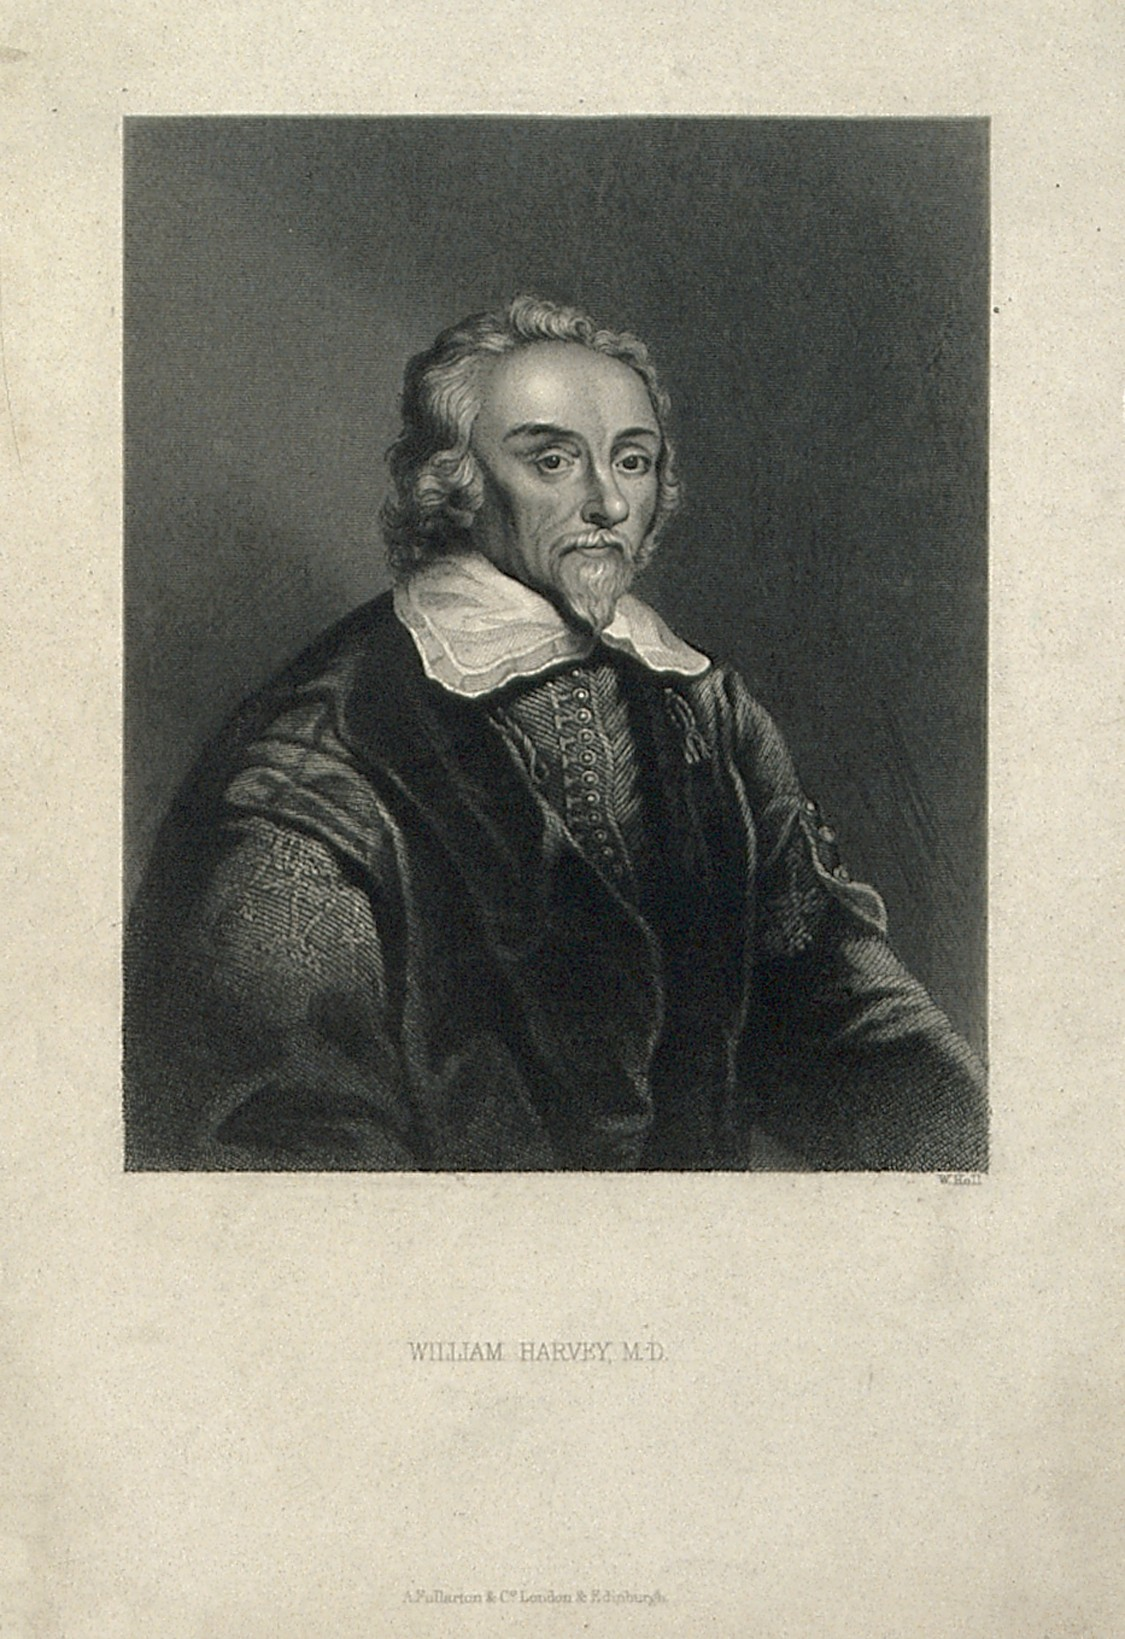
\includegraphics[width=0.3\linewidth]{images/book4/harvey.jpg}\hspace{0.05\linewidth}
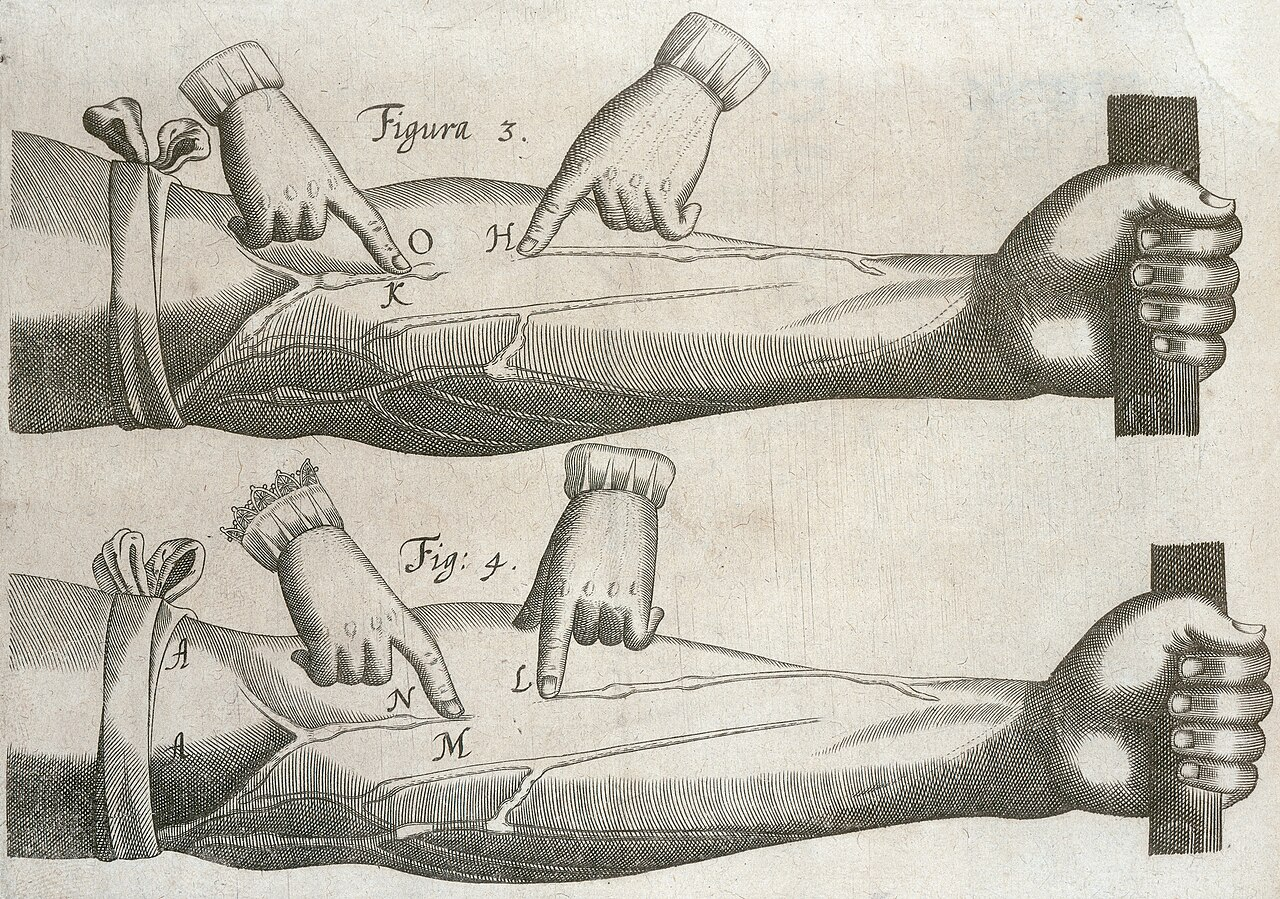
\includegraphics[width=0.42\linewidth]{images/book4/harvey-veins.jpg}

{\small وليام هارفي، واللوحة من كتابه سنة 1628:
أوردة الساعد المربوط تنتفخ أسفل الخيط، \omterm{def:b2:blood-circulation:blood}{والدم} المدفوع
نحو اليد يقف عند الدسامات.}
\end{omfigure}

\begin{omfigure}
\begin{tikzpicture}[every node/.style={font=\scriptsize}, >=stealth]
  % lungs and body
  \node[draw, rounded corners, fill=omDef!12, minimum width=3.4cm, minimum height=0.9cm] (lung) at (0,3) {الرئتان: شعيرات رئوية};
  \node[draw, rounded corners, fill=omExo!25, minimum width=3.4cm, minimum height=0.9cm] (body) at (0,-3) {الجسم: شعيرات جهازية};
  % heart chambers
  \node[draw, fill=omDef!25, minimum width=1.3cm, minimum height=0.7cm] (ra) at (-1.6,0.6) {أذين أيمن};
  \node[draw, fill=omDef!35, minimum width=1.3cm, minimum height=0.9cm] (rv) at (-1.6,-0.5) {بطين أيمن};
  \node[draw, fill=omThm!20, minimum width=1.3cm, minimum height=0.7cm] (la) at (1.6,0.6) {أذين أيسر};
  \node[draw, fill=omThm!35, minimum width=1.3cm, minimum height=0.9cm] (lv) at (1.6,-0.5) {بطين أيسر};
  \draw[->, thick] (ra) -- (rv); \draw[->, thick] (la) -- (lv);
  % pulmonary circuit
  \draw[->, very thick, omDef] (rv.west) -- ++(-1.4,0) |- (lung.west) node[pos=0.25, left, align=right] {الشريان الرئوي\\\qty{25}{mmHg}};
  \draw[->, very thick, omThm] (lung.east) -| (la.east) node[pos=0.75, right, align=left] {الأوردة الرئوية\\مؤكسجة};
  % systemic circuit
  \draw[->, very thick, omThm] (lv.east) -- ++(1.4,0) |- (body.east) node[pos=0.25, right, align=left] {الأبهر\\\qty{120}{mmHg}};
  \draw[->, very thick, omDef] (body.west) -| (ra.west);
  \node[omDef, anchor=east, align=right] at (-2.45,-1.6) {الأجوفان\\\qty{5}{mmHg}};
  \node[anchor=north, align=center] at (0,-3.7) {الجريان نفسه عبر الدارتين:\\\qty{5}{L/min} في الراحة};
\end{tikzpicture}

{\small \omterm{def:b2:blood-circulation:circuits}{الدوران المضاعف}. القلب الأيمن يرسل \omterm{def:b2:blood-circulation:blood}{الدم}
عبر الرئتين بضغط منخفض؛ والقلب الأيسر يرسله حول
الجسم بضغط عالٍ؛ والمضختان، على التوالي، تحركان الحجم
نفسه في الدقيقة.}
\end{omfigure}

\section{الأوعية وفيزياء الجريان}

\begin{definition}[الشجرة الوعائية]\label{def:b2:blood-circulation:vessels}
\index{شريان}\index{شريين}\index{شعيرة}\index{وريد}
يغادر \omterm{def:b2:blood-circulation:blood}{الدم} القلب عبر \emph{الشرايين}: وهي أنابيب سميكة الجدار
بطبقات مرنة تتمدد عند كل نبضة وترتد بين
النبضات، فتنعّم النبضات جريانًا أثبت (والأبهر
\qty{2.5}{cm} عرضًا). وتتفرع إلى \emph{شرينات}، وهي أوعية
بعُشر مليمتر أو أقل جدرانها في معظمها عضل
أملس: فالشريّن بانقباضه أو ارتخائه يغير نصف قطره
ومن ثم مقاومته تغييرًا قويًا --- فالشرينات صنابير
الدوران وموضع معظم هبوط الضغط. وهذه
تنفتح على \emph{شعيرات}: أنابيب من خلية بطانية واحدة
ملفوفة حول لمعة من \qtyrange{5}{10}{\micro m}، بطول نحو
\qty{1}{mm}، عددها نحو أربعين مليارًا بسطح كلي
قريب من \qty{600}{m^2}، ويقع عبر جدرانها كل تبادل.
وتصب الشعيرات في وُرينات و\emph{أوردة}: رقيقة الجدار
قابلة للتمدد، تحمل ثلثي \omterm{def:b2:blood-circulation:blood}{الدم} بضغط منخفض، ولها
دسامات تبقي الجريان نحو القلب بينما تعصرها العضلات.
وكل وعاء مبطن بطبقة واحدة من
\emph{البطانة}، وهي ليست بطانة سلبية بل غدة ---
إذ تطلق أكسيد النتريك لإرخاء الشريّن، وإشارات
تجنّد الكريات البيض --- ومرشحًا.
\end{definition}

\begin{omfigure}
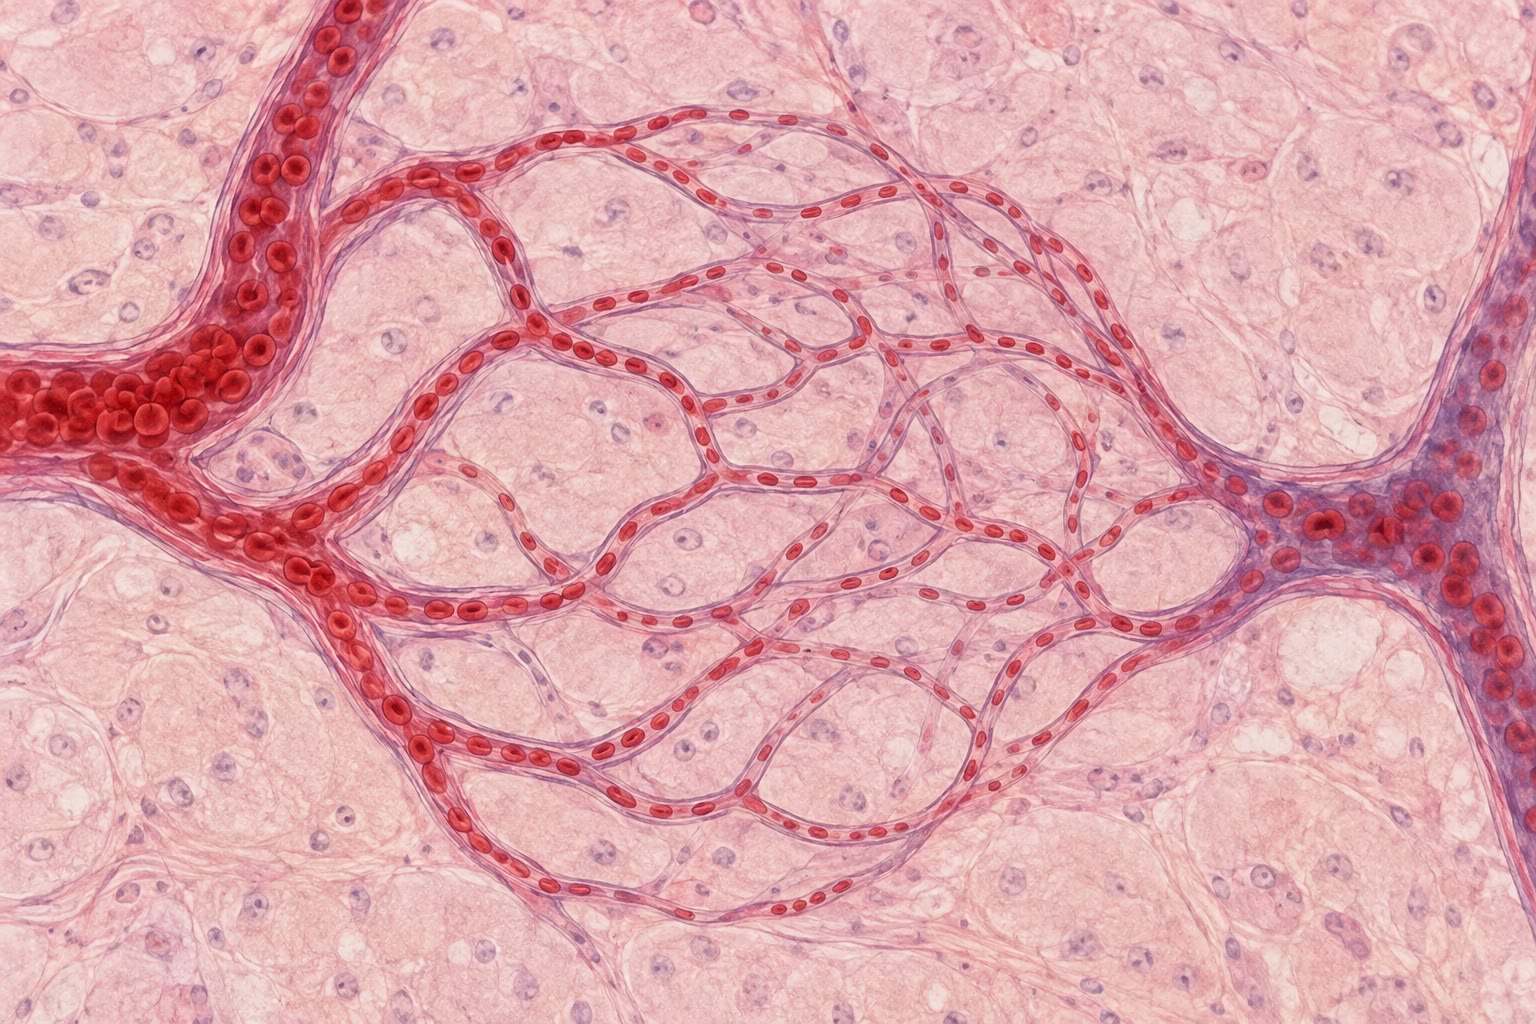
\includegraphics[width=0.55\linewidth]{images/book4/ai/b4-16-capillary-bed.jpg}

{\small سرير شعيري: \omterm{def:b2:blood-circulation:vessels}{شريّن} يغذي شبكة من الشعيرات
تسير فيها الكريات الحمر في صف واحد، ثم تتجمع في وُرين.}
\end{omfigure}

\begin{theorem}[قانون بوازوي والمقاومة الوعائية]\label{thm:b2:blood-circulation:poiseuille}
\index{قانون بوازوي}\index{مقاومة وعائية}
الجريان المستقر $Q$ لمائع لزوجته $\eta$ عبر أنبوب
نصف قطره $r$ وطوله $L$ تحت فرق ضغط $\Delta P$
هو
\[
Q = \frac{\pi r^{4}}{8\eta L}\,\Delta P, \qquad \text{ومنه}\qquad
R \equiv \frac{\Delta P}{Q} = \frac{8\eta L}{\pi r^{4}} .
\]
فالمقاومة تهبط كالقوة \emph{الرابعة} لنصف القطر: \omterm{def:b2:blood-circulation:vessels}{فالشريّن}
الذي يضيّق نصف قطره \qty{20}{\%} يضرب
مقاومته في $1/0.8^{4} = 2.4$، والذي ينصّفه يضربها في 16. وهذا
سبب استطاعة بضعة مليمترات من عضل \omterm{def:b2:blood-circulation:vessels}{الشرينات} إعادة توجيه
\omterm{def:b2:blood-circulation:blood}{دم} الجسم كله --- إلى المعي بعد وجبة، وإلى العضلات
في الجهد، وإلى الجلد في الحر --- وسبب هبوط الضغط من
\qty{95}{mmHg} في الشرايين الصغيرة إلى \qty{35}{mmHg} عند
مدخل الشعيرات، وكله تقريبًا عبر
\omterm{def:b2:blood-circulation:vessels}{الشرينات}، في حين أن الهبوط على امتداد الأبهر كسر من
مليمتر زئبق.
\end{theorem}
\begin{proof}
في الجريان الصفحي المستقر يتحرك المائع في قشور متحدة المركز؛ و
القوة اللزجة بين القشور توازن الضغط. فمن أجل
أسطوانة نصف قطرها $s < r$ تساوي قوة الضغط $\pi s^{2}\Delta P$
قوةَ الجرّ اللزج على سطحها $2\pi s L\,\eta\,(-\mathrm{d}v/
\mathrm{d}s)$، ومنه $\mathrm{d}v/\mathrm{d}s = -s\Delta P/(2\eta L)$
ومع $v(r) = 0$ يكون $v(s) = (\Delta P/4\eta L)(r^{2} - s^{2})$ --- أي
منحًى قطعيًا مكافئًا. وبمكاملة السرعة على المقطع،
$Q = \int_{0}^{r} v\,2\pi s\,\mathrm{d}s = (\pi\Delta P/2\eta L)
\int_{0}^{r}(r^{2}s - s^{3})\,\mathrm{d}s = \pi r^{4}\Delta P/8\eta
L$. (\omterm{def:b2:blood-circulation:blood}{والدم} ليس مائعًا بسيطًا تمامًا والشرايين ليست صلبة،
لكن قانون القوة الرابعة يصدق بما يكفي لإدارة جسم.)
\end{proof}

\begin{theorem}[الاستمرارية: أين يبطئ الدم]\label{thm:b2:blood-circulation:continuity}
\index{معادلة الاستمرارية}
يمر الحجم نفسه في الثانية بكل مستوى من الشجرة، فتكون
السرعة المتوسطة عند مستوى $v = Q/A$، حيث $A$ هو مساحة المقطع
\emph{الكلية} لكل الأوعية في ذلك المستوى. فالأبهر
(\qty{3}{cm^2}) يحمل \qty{5}{L/min} بسرعة \qty{28}{cm/s}؛ و
الشعيرات، بمقطع كلي قريب من \qty{3000}{cm^2}، تحمله
بسرعة \qty{0.03}{cm/s}، فتستغرق \omterm{def:b2:blood-circulation:blood}{الكرية الحمراء} نحو ثلاث ثوانٍ
لعبور \omterm{def:b2:blood-circulation:vessels}{شعيرة} --- وهو زمن يكفي لينتشر أكسجينها خارجًا
(\cref{ch:b2:unicellular-diversity}: أي ميكرومتر في
ميلي ثانية). والأوردة، ومقطعها الكلي أصغر من مقطع
الشعيرات، تسرّع \omterm{def:b2:blood-circulation:blood}{الدم} من جديد إلى \qty{10}{cm/s} في
الأجوفين. فالشجرة مبنية بحيث يكون \omterm{def:b2:blood-circulation:blood}{الدم} بطيئًا بالضبط حيث
يجب أن يتبادل وسريعًا في كل مكان آخر.
\end{theorem}
\begin{proof}
حفظ الحجم: فما يدخل مستوًى في الثانية يغادره،
فيكون $Q = A\,v$ نفسه في كل مستوى. و$\qty{5}{L/min} =
\qty{83}{cm^3/s}$؛ و$83/3 = \qty{28}{cm/s}$؛ و$83/3000 =
\qty{0.028}{cm/s}$.
\end{proof}

\begin{omfigure}
\begin{tikzpicture}
\begin{axis}[
  width=0.9\linewidth, height=6.4cm,
  axis x line=bottom, axis y line=left,
  xmin=0, xmax=7, ymin=0, ymax=130,
  xtick={0.5,1.5,2.5,3.5,4.5,5.5,6.5},
  xticklabels={الأبهر, شرايين, شرينات, شعيرات, وريدات, أوردة, أجوفان},
  x tick label style={font=\scriptsize, rotate=30, anchor=north east},
  ylabel={الضغط (\unit{mmHg})}, ylabel style={font=\small, omThm},
  tick label style={font=\small}, ytick={0,40,80,120},
  legend style={font=\scriptsize, at={(0.97,0.95)}, anchor=north east, draw=none},
  clip=false,
]
\addplot[very thick, omThm] coordinates {(0,120) (0.5,118) (1,110) (1.5,100) (2,95) (2.5,60) (3,35) (3.5,25) (4,15) (4.5,12) (5,8) (5.5,5) (6,4) (6.5,3) (7,2)};
\addlegendentry{الضغط المتوسط}
\addplot[very thick, omThm, dashed] coordinates {(0,120) (0.5,120) (1,125) (1.5,120) (2,100)};
\addplot[very thick, omThm, dashed] coordinates {(0,80) (0.5,80) (1,80) (1.5,82) (2,88)};
\addlegendentry{الانقباضي والانبساطي}
\end{axis}
\begin{axis}[
  width=0.9\linewidth, height=6.4cm,
  axis x line=none, axis y line=right,
  xmin=0, xmax=7, ymin=0, ymax=32,
  ylabel={السرعة (\unit{cm/s})}, ylabel style={font=\small, omDef},
  tick label style={font=\small}, ytick={0,10,20,30},
  legend style={font=\scriptsize, at={(0.97,0.72)}, anchor=north east, draw=none},
  clip=false,
]
\addplot[very thick, omDef] coordinates {(0,28) (0.5,26) (1,18) (1.5,10) (2,5) (2.5,1.5) (3,0.3) (3.5,0.03) (4,0.3) (4.5,1.5) (5,4) (5.5,7) (6,9) (6.5,10) (7,10)};
\addlegendentry{السرعة المتوسطة}
\end{axis}
\end{tikzpicture}

{\small الضغط (بالأحمر) والسرعة المتوسطة (بالأزرق) على امتداد \omterm{def:b2:blood-circulation:circuits}{الدوران
الجهازي}. تُنعَّم النبضة في الشرايين، ويهبط الضغط
في معظمه عبر \omterm{def:b2:blood-circulation:vessels}{الشرينات}، ويكون \omterm{def:b2:blood-circulation:blood}{الدم} أبطأ ما يكون في
الشعيرات، حيث يكون المقطع الكلي ألف ضعف مقطع
الأبهر.}
\end{omfigure}

\begin{theorem}[الشريان المرن خزانًا]\label{thm:b2:blood-circulation:windkessel}
\index{خزان مرن}\index{مطاوعة!شريانية}\index{ضغط النبض}
يقذف القلب دفقات؛ وتتلقى الأنسجة جريانًا شبه
ثابت. والشرايين الكبيرة هي التي تنعّم: فهي تتمدد خلال
القذف، فتخزن جزءًا من حجم الضربة، وترتد خلال
الانبساط فتدفعه. فإذا كان للشرايين \emph{مطاوعة}
$C$ (أي حجم مخزون لكل وحدة ضغط) وللشرينات
مقاومة $R$، فإن الضغط يتناقص خلال الانبساط، والدسام الأبهري مغلق،
وفق
\[
P(t) = P_{s}\,e^{-t/RC},
\]
فيكون الضغط الانبساطي بعد انبساط مدته $t_d$
هو $P_s e^{-t_d/RC}$: فمع $R = \qty{1}{mmHg.s/mL}$، و$C =
\qty{2}{mL/mmHg}$، و$t_d = \qty{0.8}{s}$، يهبط انقباضي
\qty{120}{mmHg} إلى \qty{80}{mmHg}. والأبهر الأقسى (وقيمة $C$ فيه أصغر،
كما في الشيخوخة) يدع الضغط يهبط أكثر بين النبضات
ويرتفع أعلى خلال القذف: فيتسع \emph{\omterm{thm:b2:blood-circulation:windkessel}{ضغط النبض}}،
ويعمل القلب ضد ذروة أعلى.
\end{theorem}
\begin{proof}
خلال الانبساط لا يدخل \omterm{def:b2:blood-circulation:blood}{دم} إلى الشرايين ويغادرها \omterm{def:b2:blood-circulation:blood}{الدم}
عبر \omterm{def:b2:blood-circulation:vessels}{الشرينات} عند $Q = P/R$؛ فيهبط الحجم الشرياني بمعدل
$\mathrm{d}V/\mathrm{d}t = -P/R$، ولمّا كان $\mathrm{d}V = C\,
\mathrm{d}P$، صار $C\,\mathrm{d}P/\mathrm{d}t = -P/R$، وحلها هو
الأسّي بثابت زمن $RC$. فمع $RC = \qty{2}{s}$:
$120\,e^{-0.4} = \qty{80}{mmHg}$.
\end{proof}

\section{التبادل في الشعيرات}

\begin{proposition}[نمطان من التبادل]\label{prop:b2:blood-circulation:exchange}
\index{تبادل شعيري}\index{قوى ستارلنغ}\index{وذمة}\index{لمف}
عبر جدار \omterm{def:b2:blood-circulation:vessels}{الشعيرة} تنتقل المنحلّات \emph{بالانتشار} --- فالغازات
والشحوم عبر الخلايا، والماء والمنحلّات الصغيرة عبر
الشقوق بينها، على المساحة الهائلة والمسافة القصيرة
اللتين تجعلان التدفق وافرًا (قانون فيك، كما في \omterm{def:b2:mammal-reproduction:placenta}{مشيمة}
\cref{ch:b2:mammal-reproduction}) --- وينتقل الماء
بطريق \emph{الجريان الكتلي}، مدفوعًا بموازنة ضغطين. فالضغط
الهيدروستاتي في \omterm{def:b2:blood-circulation:vessels}{الشعيرة}، $P_c$، يدفع السائل خارجًا؛ و
\omterm{thm:b2:blood-circulation:oncotic}{الضغط الغرواني} لبروتينات \omterm{def:b2:blood-circulation:blood}{البلازما}، $\pi_c$، يجذبه داخلًا
(وهي \emph{\omterm{prop:b2:blood-circulation:exchange}{قوى ستارلنغ}}). وعند الطرف الشرياني يفوق $P_c \approx
\qty{35}{mmHg}$ مقدارَ $\pi_c \approx \qty{25}{mmHg}$ فيرشح
السائل خارجًا؛ وعند الطرف الوريدي يكون $P_c \approx \qty{15}{mmHg}$ فيُعاد
امتصاص السائل؛ وعلى الجسم كله يرشح نحو \qty{20}{L} في اليوم
خارجًا ويعود \qty{17}{L}، والفرق البالغ \qty{3}{L}، مع
البروتينات التي تسربت، تجمعه الأوعية \emph{اللمفية}
وتعيده إلى الأوردة عند العنق. و\emph{الوذمة} --- أي الانتفاخ
بالسائل في الأنسجة --- تتبع كلما اختل الميزان:
ضغط وريدي عالٍ (قصور القلب)، أو بروتين \omterm{def:b2:blood-circulation:blood}{بلازما} منخفض
(المجاعة، أو مرض الكبد أو الكلية)، أو شعيرات راشحة
(الالتهاب)، أو لمفيات مسدودة.
\end{proposition}

\begin{omfigure}
\begin{tikzpicture}[every node/.style={font=\scriptsize}, >=stealth]
  % capillary
  \draw[thick, fill=omThm!10] (0,0) rectangle (9,1.2);
  \node[left] at (-0.1,0.6) {شريّن};
  \node[right] at (9.1,0.6) {وُرين};
  \draw[->, very thick, omThm] (0.3,0.6) -- (8.7,0.6);
  % pressures
  \node[above, align=center] at (1.5,1.3) {الطرف الشرياني\\$P_c = 35$، $\pi_c = 25$};
  \node[above, align=center] at (7.5,1.3) {الطرف الوريدي\\$P_c = 15$، $\pi_c = 25$};
  \foreach \x in {0.8,1.5,2.2} \draw[->, thick, omDef] (\x,0) -- (\x,-0.7);
  \node[below, align=center, omDef] at (1.5,-0.75) {الصافي $+10$ ملم زئبق:\\رشح};
  \foreach \x in {6.8,7.5,8.2} \draw[->, thick, omDef] (\x,-0.7) -- (\x,0);
  \node[below, align=center, omDef] at (7.5,-0.75) {الصافي $-10$ ملم زئبق:\\إعادة امتصاص};
  \draw[->, thick, omExo!70!black] (4.5,-0.4) -- (4.5,-1.6) node[below, align=center] {الفائض إلى اللمف:\\\qty{3}{L} في اليوم};
  \node[align=center] at (4.5,-0.15) {سائل خلالي};
\end{tikzpicture}

{\small \omterm{prop:b2:blood-circulation:exchange}{قوى ستارلنغ} على امتداد \omterm{def:b2:blood-circulation:vessels}{شعيرة}. الضغط الهيدروستاتي
يدفع السائل خارجًا \omterm{thm:b2:blood-circulation:oncotic}{والضغط الغرواني} لبروتينات \omterm{def:b2:blood-circulation:blood}{البلازما} يجذبه
راجعًا؛ والرشح عند الطرف الشرياني يفوق إعادة الامتصاص عند
الطرف الوريدي، واللمف يعيد الفرق.}
\end{omfigure}

\begin{theorem}[الضغط الغرواني]\label{thm:b2:blood-circulation:oncotic}
\index{ضغط غرواني}\index{ألبومين}
محلول فيه $c$ مولًا في اللتر من منحلّ لا يستطيع عبور
غشاء يمارس عبره ضغطًا تناضحيًا $\pi = cRT$ (قانون فانت
هوف). وألبومين \omterm{def:b2:blood-circulation:blood}{البلازما}، وهو \qty{40}{g/L} من بروتين كتلته المولية
\qty{66}{kg/mol}، يساوي $c = \qty{0.6}{mmol/L}$ ويعطي $\pi =
0.6\times 8.314\times 310 = \qty{1.55}{kPa} \approx \qty{12}{mmHg}$؛
وتبلغ البروتينات الأخرى والشوارد الزائدة التي تحتجزها شحنة
الألبومين السالبة بالمجموع نحو \qty{25}{mmHg}. أما كلوريد
الصوديوم في \omterm{def:b2:blood-circulation:blood}{البلازما}، عند \qty{150}{mmol/L}، فكان ليمارس
\qty{5800}{mmHg} --- لكنه يعبر جدار \omterm{def:b2:blood-circulation:vessels}{الشعيرة} بحرية فلا
يمارس شيئًا عبره. والذي يهم \omterm{def:b2:blood-circulation:vessels}{الشعيرة} هو
البروتين: فنصّف الألبومين، كما في مرض كلية يفقده في
البول، ينتصف الجذب المعيد للامتصاص، ويتراكم السائل في
الأنسجة، وينتفخ المريض.
\end{theorem}
\begin{proof}
$\qty{40}{g/L}/\qty{66000}{g/mol} = \qty{6.1e-4}{mol/L} =
\qty{0.61}{mol/m^3}$؛ و$\pi = cRT = 0.61\times 8.314\times 310 =
\qty{1570}{Pa}$؛ و$\qty{1}{mmHg} = \qty{133}{Pa}$، ومنه \qty{11.8}{mmHg}.
أما قانون فانت هوف نفسه فهو حد المحلول المخفف المشتق في
مجلد السنة الأولى.
\end{proof}

\begin{example}[الدوران جملةَ نقل]\label{ex:b2:blood-circulation:transport}
خمسة لترات في الدقيقة عبر \qty{600}{m^2} من جدار الشعيرات خدمة
توصيل لا نظير لها. فهي تجلب لكل خلية أكسجينًا في حدود
بضعة أقطار خلوية (فلا خلية في الجسم تبعد أكثر من
\qty{20}{\micro m} عن \omterm{def:b2:blood-circulation:vessels}{شعيرة})، وتزيل $\mathrm{CO_2}$ عنها،
واللاكتات والبولة، وتحمل غلوكوز الكبد إلى الدماغ و
حموض مخازن الشحم الدهنية إلى العضلات، وتوزع
هرمونات \cref{ch:b2:cell-signalling} من غدة واحدة إلى كل
مستقبل في الجسم في دقيقة، وتنقل حرارة اللب إلى
الجلد وبالعكس، وتنقل الكريات البيض إلى جرح في غضون
ساعات. وهي كذلك موضع الضعف: فخثرة أو نزف أو مضخة
عاطلة توقف ذلك كله دفعة واحدة، والدماغ، الذي لا يخزن
وقودًا، يخفق في ثوان. وبقية هذا الجزء من الكتاب
عن المضخة (\cref{ch:b2:heart}) وعن كيف يُنظَّم الضغط
لتستمر الخدمة عبر النهوض والعدو والنزف
(\cref{ch:b2:blood-pressure}).
\end{example}

\section{تمارين}

\begin{exercise}[$\star$]\label{exo:b2:blood-circulation:1}
أعط تركيب \omterm{def:b2:blood-circulation:blood}{الدم} بالحجم وعدد كل مكوّن خلوي وقياسه و
وظيفته.
\end{exercise}

\begin{exercise}[$\star$]\label{exo:b2:blood-circulation:2}
ارسم دارة سمكة ودارة ثديي، وأشّر الضغوط، و
قل ماذا تكسب الدارة المضاعفة.
\end{exercise}

\begin{exercise}[$\star$]\label{exo:b2:blood-circulation:3}
من أجل كل صنف وعائي --- \omterm{def:b2:blood-circulation:vessels}{شريان}، \omterm{def:b2:blood-circulation:vessels}{وشريّن}، \omterm{def:b2:blood-circulation:vessels}{وشعيرة}، \omterm{def:b2:blood-circulation:vessels}{ووريد} --- أعط
بنية الجدار والوظيفة التي يخدمها.
\end{exercise}

\begin{exercise}[$\star$]\label{exo:b2:blood-circulation:4}
أعد بناء حجة هارفي من الكمية، بأرقام حديثة:
\qty{70}{mL} في النبضة، و\num{72} نبضة في الدقيقة، و\qty{5}{L} من \omterm{def:b2:blood-circulation:blood}{الدم}.
\end{exercise}

\begin{exercise}[$\star\star$]\label{exo:b2:blood-circulation:5}
احسب هبوط الضغط على امتداد الأبهر (نصف القطر \qty{1.25}{cm}،
والطول \qty{40}{cm}، و$\eta = \qty{3e-3}{Pa.s}$) وهو يحمل
\qty{5}{L/min} \omterm{thm:b2:blood-circulation:poiseuille}{بقانون بوازوي}، بالباسكال وبملم الزئبق. وعلّق.
\end{exercise}

\begin{exercise}[$\star\star$]\label{exo:b2:blood-circulation:6}
\omterm{def:b2:blood-circulation:vessels}{شريّن} نصف قطره \qty{15}{\micro m} ينقبض إلى
\qty{12}{\micro m}، ثم يتوسع إلى \qty{20}{\micro m}. فبأي
عامل تتغير مقاومته في كل حالة، وجريانه عند
ضغط ثابت؟
\end{exercise}

\begin{exercise}[$\star\star$]\label{exo:b2:blood-circulation:7}
للأبهر مقطع \qty{3}{cm^2} وللشعيرات مقطع
كلي \qty{3000}{cm^2}؛ والجريان \qty{5}{L/min}. احسب
السرعة المتوسطة في كل منهما، والزمن الذي تقضيه \omterm{def:b2:blood-circulation:blood}{كرية حمراء} في
\omterm{def:b2:blood-circulation:vessels}{شعيرة} \qty{1}{mm}. وفي الجهد يرتفع النتاج إلى
\qty{25}{L/min} وتنفتح شعيرات العضل: فماذا يحدث
لزمن العبور؟
\end{exercise}

\begin{exercise}[$\star\star$]\label{exo:b2:blood-circulation:8}
مع $P_c = 35$ و\qty{15}{mmHg} عند الطرفين، و$\pi_c =
\qty{25}{mmHg}$، والضغوط الخلالية مهملة، احسب ضغط
الرشح الصافي عند كل طرف. وماذا يحدث إذا ارتفع الضغط الوريدي
حتى صار $P_c$ عند الطرف الوريدي \qty{28}{mmHg}؟
\end{exercise}

\begin{exercise}[$\star\star$]\label{exo:b2:blood-circulation:9}
احسب \omterm{thm:b2:blood-circulation:oncotic}{الضغط الغرواني} عند \qty{40}{g/L} من الألبومين
(\qty{66}{kg/mol}) عند \qty{37}{\celsius}، وعند \qty{20}{g/L}. ولماذا
لا يسهم صوديوم \omterm{def:b2:blood-circulation:blood}{البلازما}، عند \qty{150}{mmol/L}، بشيء
في ميزان ستارلنغ؟
\end{exercise}

\begin{exercise}[$\star\star\star$]\label{exo:b2:blood-circulation:10}
مع $R = \qty{1}{mmHg.s/mL}$ و$C = \qty{2}{mL/mmHg}$، احسب
الضغط الانبساطي بعد \qty{0.8}{s} من انقباضي قدره
\qty{120}{mmHg}. وأعد الحساب من أجل أبهر مطاوعته النصف. واشرح لماذا
يكون ضغط نبض المسنين واسعًا، وما يكلفه ذلك
القلب.
\end{exercise}

\begin{exercise}[$\star\star\star$]\label{exo:b2:blood-circulation:11}
المقاومة الجهازية $R = (P_{\text{شرياني}} - P_{\text{وريدي}})/Q$.
احسبها في الراحة ($95 - 5$ ملم زئبق، و\qty{5}{L/min}) وفي الجهد
($110 - 5$، و\qty{25}{L/min}). وبأي عامل تغير متوسط نصف قطر
\omterm{def:b2:blood-circulation:vessels}{الشرينات}، إذا حملت \omterm{def:b2:blood-circulation:vessels}{الشرينات} المقاومة كلها؟
\end{exercise}

\begin{exercise}[$\star\star\star$]\label{exo:b2:blood-circulation:12}
«الدوران مبني بحيث يكون \omterm{def:b2:blood-circulation:blood}{الدم} بطيئًا حيث يجب أن
يتبادل وسريعًا في كل مكان آخر.» ناقش، \omterm{thm:b2:blood-circulation:continuity}{بمعادلة
الاستمرارية} \omterm{thm:b2:blood-circulation:poiseuille}{وقانون بوازوي} وهندسة الشجرة، وقل
لماذا لا يستطيع \omterm{def:b2:blood-circulation:circuits}{دوران مفتوح} فعل الشيء نفسه.
\end{exercise}

\section{مسألة: الدوران بالأرقام}

\begin{problem}[{مسألة نهاية الأسبوع --- إعادة حساب هارفي، وحساب ضغوط
شجرة الأوعية وسرعاتها ببوازوي والاستمرارية،
وموازنة رشح الشعيرات اليومي، ونمذجة تنعيم
الأبهر، وتنتهي إلى النتاج القلبي، وهبوط الضغط الشرييني،
ورشح اليوم، والضغط الانبساطي}]
\label{pb:b2:blood-circulation:1}
المعطيات: حجم الضربة \qty{70}{mL}، ومعدل القلب \qty{72}{min^{-1}}،
وحجم \omterm{def:b2:blood-circulation:blood}{الدم} \qty{5}{L}، و$\eta = \qty{3e-3}{Pa.s}$، و$\qty{1}{mmHg} =
\qty{133}{Pa}$. والأبهر: نصف القطر \qty{1.25}{cm}، والطول \qty{40}{cm}.
\omterm{def:b2:blood-circulation:vessels}{والشرينات}: $3\times 10^{6}$ على التوازي، نصف قطر كل منها
\qty{15}{\micro m} وطوله \qty{1}{mm}. والشعيرات: $4\times
10^{10}$، بنصف قطر \qty{3}{\micro m}، وطول \qty{1}{mm}، وربعها
مفتوح في الراحة. وستارلنغ: $P_c$ من 35 إلى \qty{15}{mmHg} على امتداد
\omterm{def:b2:blood-circulation:vessels}{شعيرة}، و$\pi_c = \qty{25}{mmHg}$. \omterm{thm:b2:blood-circulation:windkessel}{والخزان المرن}: $C =
\qty{2}{mL/mmHg}$، والانبساط \qty{0.8}{s}.

\medskip
\noindent\textbf{الجزء الأول --- حساب هارفي.}
\begin{enumerate}
  \item احسب النتاج القلبي باللترات في الدقيقة وفي اليوم.
  \item كم مرة يدور حجم \omterm{def:b2:blood-circulation:blood}{الدم} في اليوم؟
  \item كان تقدير هارفي أوقيتين (\qty{57}{g}) في النبضة،
        افترض أن ربعها على الأقل يُقذف، عند 72 نبضة
        في الدقيقة. فأي كتلة من \omterm{def:b2:blood-circulation:blood}{الدم} أعطى ذلك في الساعة، وكيف
        قارنها بوزن رجل؟
  \item لماذا كانت هذه حجة على الدوران لا على
        الإنتاج والاستهلاك المستمرين؟
  \item صف تجربة الرباط وما بيّنته الدسامات.
  \item ما الذي لم يستطع هارفي رؤيته، ومن رآه؟
\end{enumerate}

\medskip
\noindent\textbf{الجزء الثاني --- الشجرة.}
\begin{enumerate}[resume]
  \item احسب السرعة المتوسطة في الأبهر.
  \item احسب هبوط الضغط على امتداد الأبهر \omterm{thm:b2:blood-circulation:poiseuille}{بقانون بوازوي}،
        بملم الزئبق.
  \item احسب مقاومة \omterm{def:b2:blood-circulation:vessels}{شريّن} واحد ومقاومة $3\times
        10^{6}$ منها على التوازي.
  \item احسب هبوط الضغط عبر \omterm{def:b2:blood-circulation:vessels}{الشرينات} عند
        النتاج في الراحة، بملم الزئبق.
  \item احسب المقطع الكلي للشعيرات المفتوحة و
        السرعة المتوسطة فيها؛ ثم زمن العبور عبر واحدة.
  \item تنقبض \omterm{def:b2:blood-circulation:vessels}{الشرينات} فيهبط نصف قطرها
        \qty{10}{\%}. أعد حساب الهبوط. وماذا على القلب أن يفعل
        ليبقي النتاج نفسه؟
\end{enumerate}

\medskip
\noindent\textbf{الجزء الثالث --- الشعيرات.}
\begin{enumerate}[resume]
  \item احسب ضغط الرشح الصافي عند الطرف الشرياني، وعند
        الطرف الوريدي، وعند المنتصف (اعتبر أن $P_c$ يهبط
        خطيًا).
  \item اقسم \omterm{def:b2:blood-circulation:vessels}{الشعيرة} إلى النصف الراشح و
        النصف المعيد للامتصاص وقدّر السائل المرشَّح و
        المعاد امتصاصه في اليوم على الجسم كله، آخذًا الضغطين
        الصافيين المتوسطين على كل نصف $+10$ و
        \qty{-8.5}{mmHg} وكل نصف يحرك \qty{2}{L} في اليوم لكل
        ملم زئبق.
  \item استنتج جريان اللمف.
  \item يهبط ألبومين \omterm{def:b2:blood-circulation:blood}{البلازما} إلى \qty{20}{g/L}. أعد حساب $\pi_c$
        (وافترض أنه يتقيّس مع الألبومين) والضغوط الصافية عند
        الطرفين. فماذا يحدث؟
  \item يرتفع الضغط الوريدي فيصير $P_c$ من 35 إلى
        \qty{28}{mmHg}. أعد حساب الضغط الصافي المتوسط و
        الميزان اليومي. وأين يذهب السائل؟
  \item احسب السطح الشعيري الكلي (أسطوانات، وكلها)
        والزمن الذي تستغرقه جزيئة لتنتشر إلى خلية تبعد
        \qty{20}{\micro m} عن \omterm{def:b2:blood-circulation:vessels}{شعيرة} ($D = \qty{1e-9}{m^2/s}$).
\end{enumerate}

\medskip
\noindent\textbf{الجزء الرابع --- الأبهر خزانًا.}
\begin{enumerate}[resume]
  \item احسب المقاومة الجهازية من ضغط متوسط قدره
        \qty{93}{mmHg}، وضغط وريدي \qty{3}{mmHg}، والنتاج في الراحة،
        بوحدة \unit{mmHg.s/mL}.
  \item احسب ثابت الزمن $RC$ والضغط الانبساطي
        بعد \qty{0.8}{s} من انقباضي قدره \qty{120}{mmHg}.
  \item أعد الحساب من أجل $C = \qty{1}{mL/mmHg}$. فماذا حدث
        \omterm{thm:b2:blood-circulation:windkessel}{لضغط النبض}؟
  \item يرتفع معدل القلب إلى \num{120} ويقصر الانبساط إلى
        \qty{0.3}{s}. احسب الضغط الانبساطي.
  \item من \qty{70}{mL} المقذوفة، كم يُخزن في
        الشرايين خلال الانقباض إذا ارتفع الضغط
        \qty{20}{mmHg}؟ وأين يذهب الباقي؟
  \item اشرح لماذا تعتمد الشرايين الإكليلية، التي تمتلئ في الانبساط،
        على ارتداد الأبهر.
  \item اذكر النتيجة: النتاج القلبي، وهبوط الضغط
        الشرييني، والرشح الصافي في اليوم، والضغط الانبساطي
        من أجل $C = 2$ و$C = 1$.
\end{enumerate}
\end{problem}
